
\begin{figure}[t!]
\captionsetup[subfigure]{}

\begin{tabular}{@{}c@{}}

\begin{subfigure}{\leftwidth}
  {\vspace{\titleoffset}{\textbf{\mbox{Overview}} \\ \textbf{\mbox{patterns}} \\ { \small (Sec.\ \ref{s:related_work_overview})}} }
  \label{f:overview}
\end{subfigure}
\begin{subfigure}{\familypicwidthPlus}
  \centering
  % include second image
  \fbox{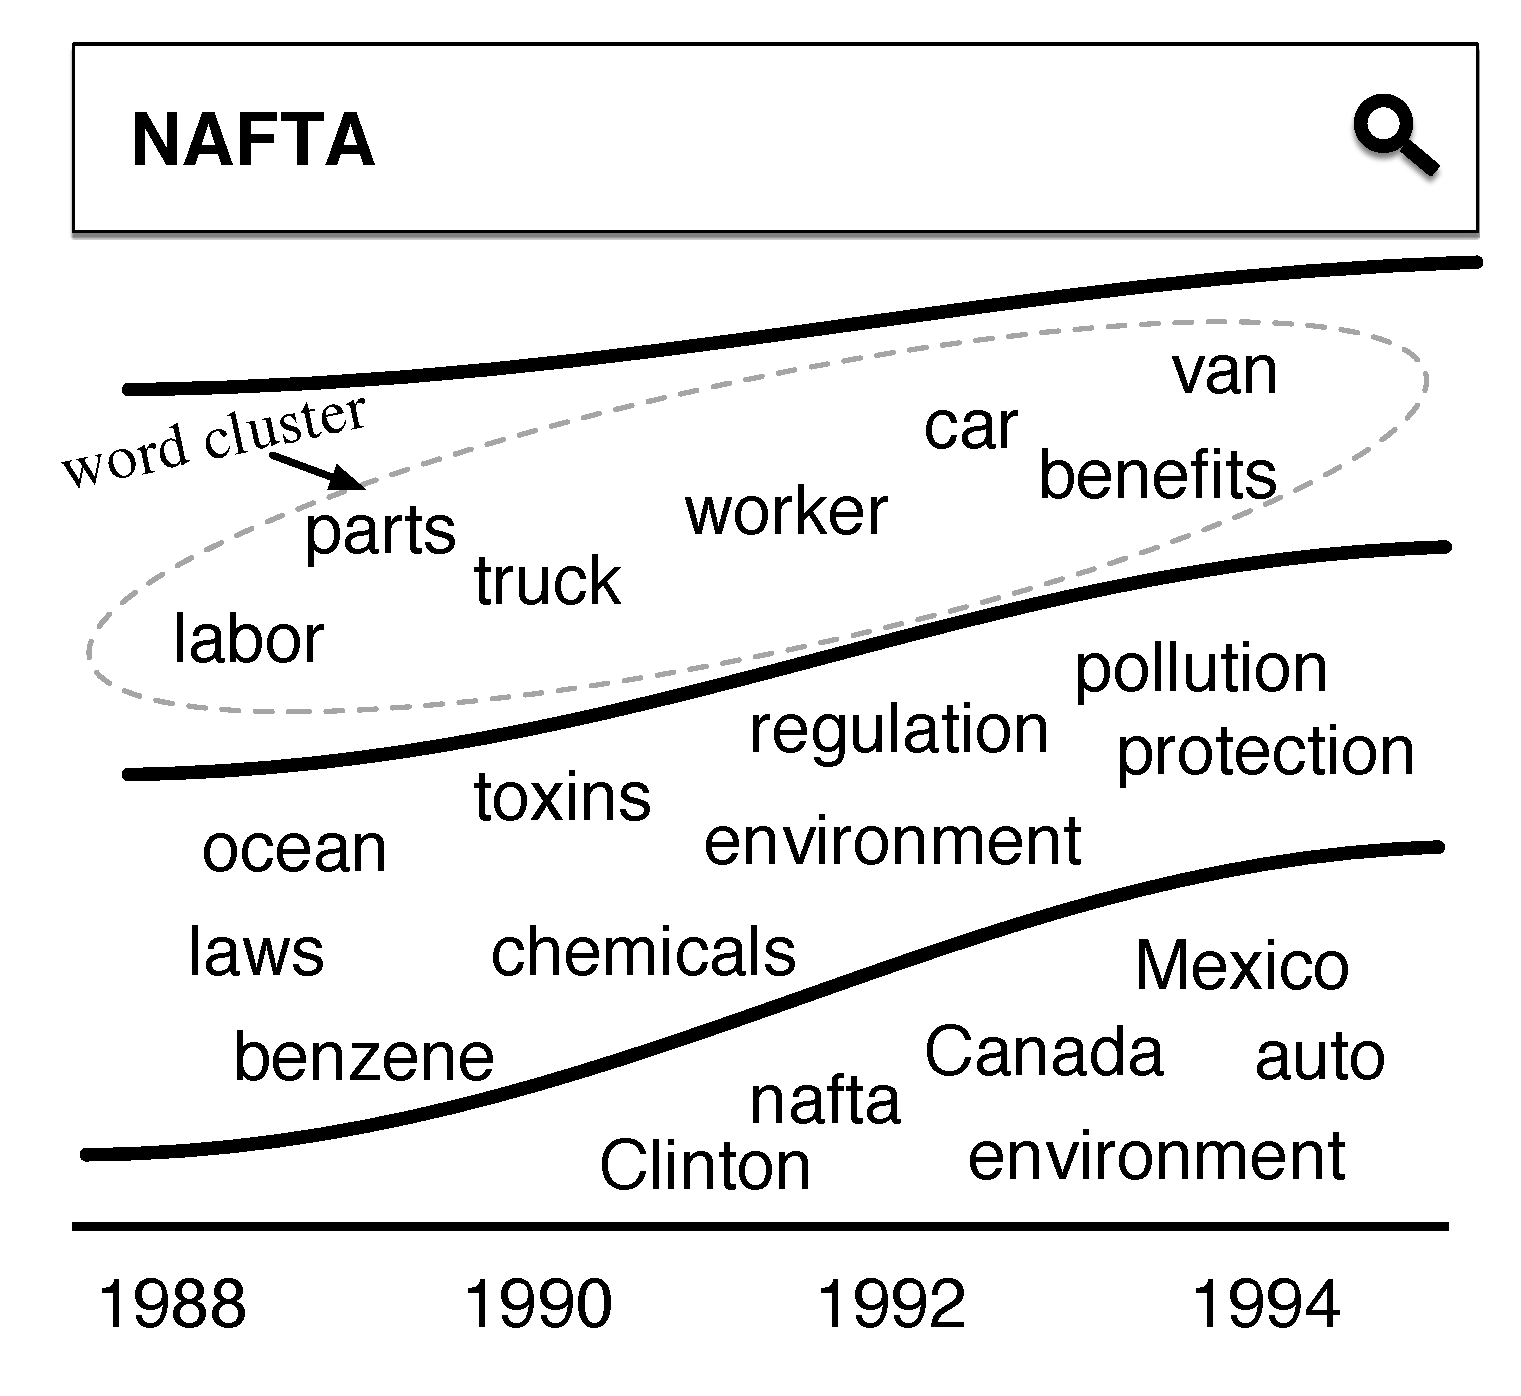
\includegraphics[width=\familypicwidth]{figures/families/clustering.pdf}}
  \caption{\hspace{.4cm}{\small Word clustering (Section \ref{s:word_clustering_family})} \\ \centerline{ \footnotesize Examples: \cite{HierarchicalTopics,overview,termite, tiisclusterone, tiisclustertwo, tiisclusterthree}}  }
  \label{f:wordclustering_family}
\end{subfigure} 
\begin{subfigure}{\familypicwidthPlus}
  \centering
  % include first image \hspace{.35cm} 
  \fbox{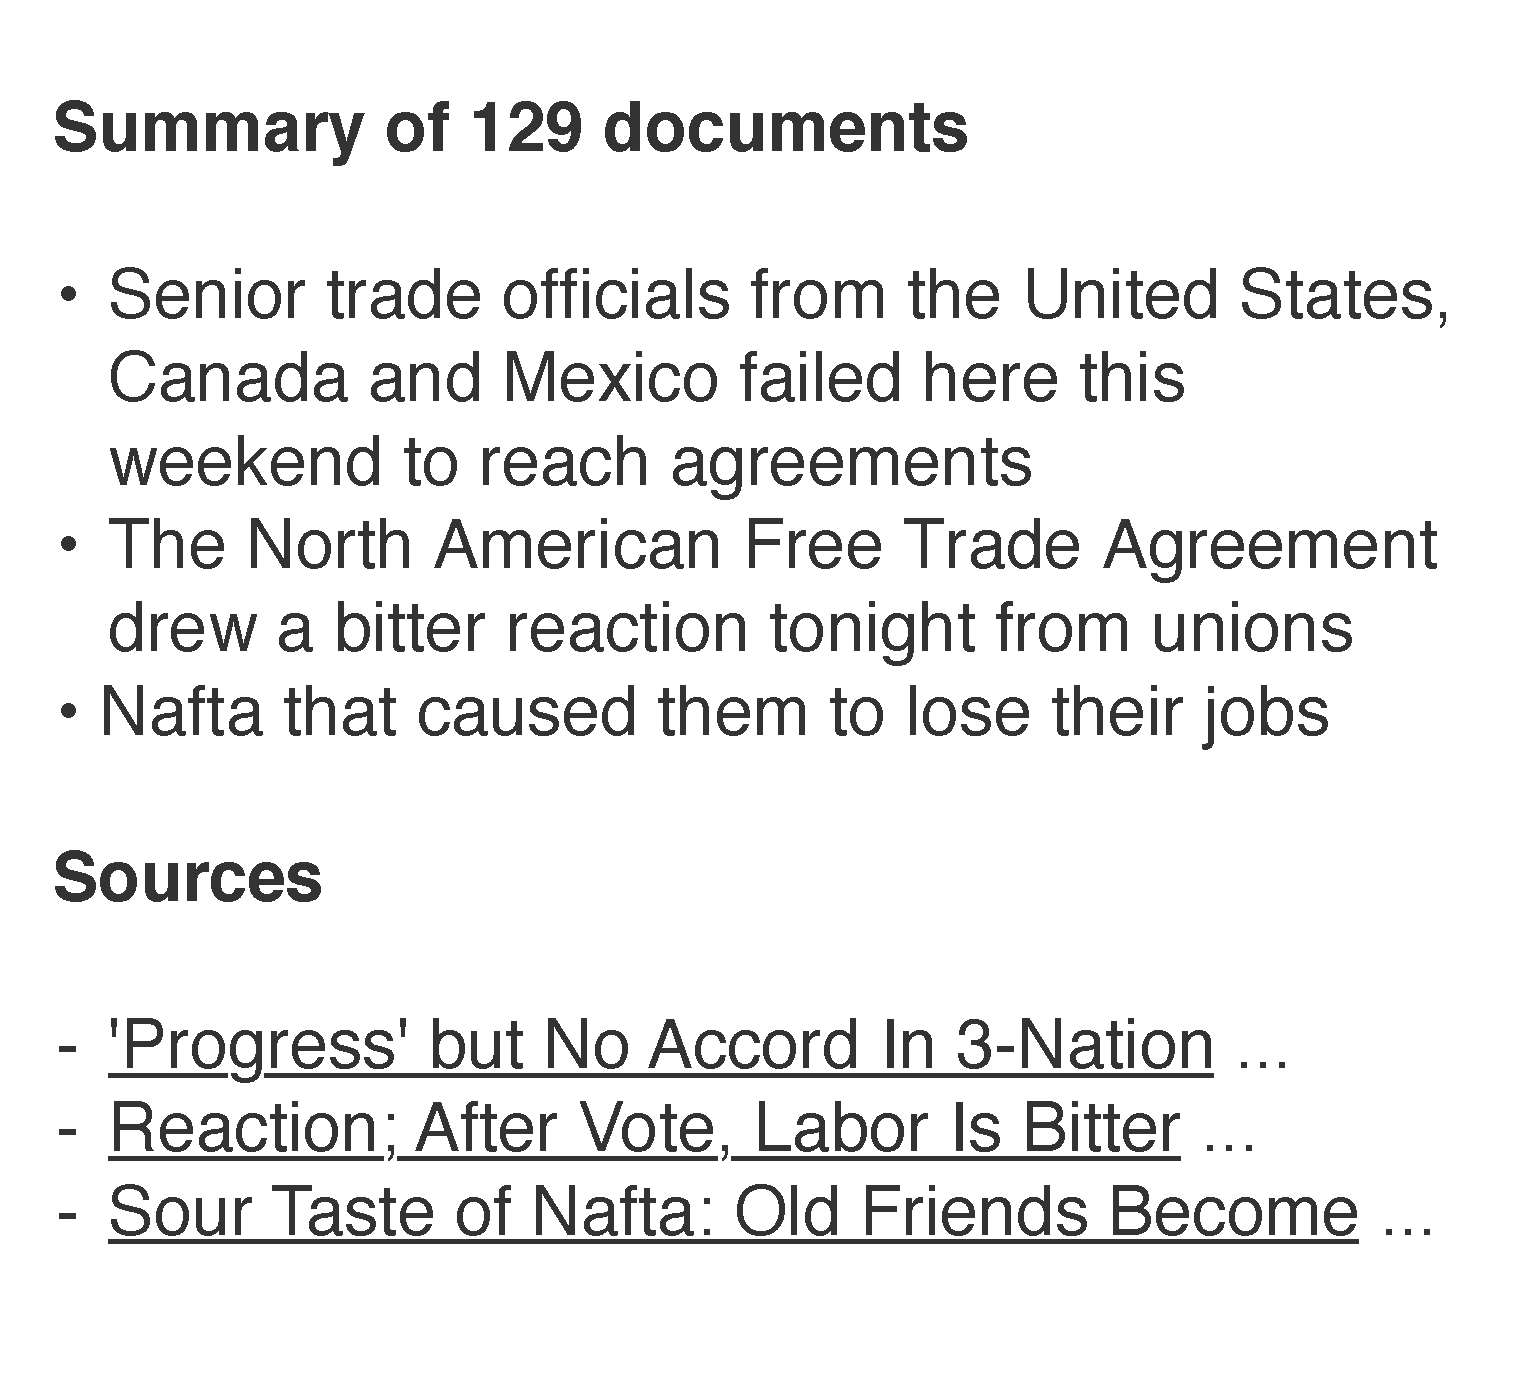
\includegraphics[width=\familypicwidth]{figures/families/summarization.pdf}}\hspace*{-0cm}
  \hspace{.7cm}\caption{\hspace{.0cm} {\small Textual \& visual summary (Sec.\ \ref{s:textual_summary_family})} \\ { \centerline{\footnotesize  \centerline {Examples: \cite{NewsblasterMain, summons, bambrick-etal-2020-nstm} }}}}
  \label{f:textual_summary_family}
\end{subfigure} \\ \\
\begin{subfigure}{1.5cm}
  \textbf{}
\end{subfigure}
%\begin{subfigure}{\familypicwidthPlus}
%  \centering
%  % include first image
%  \fbox{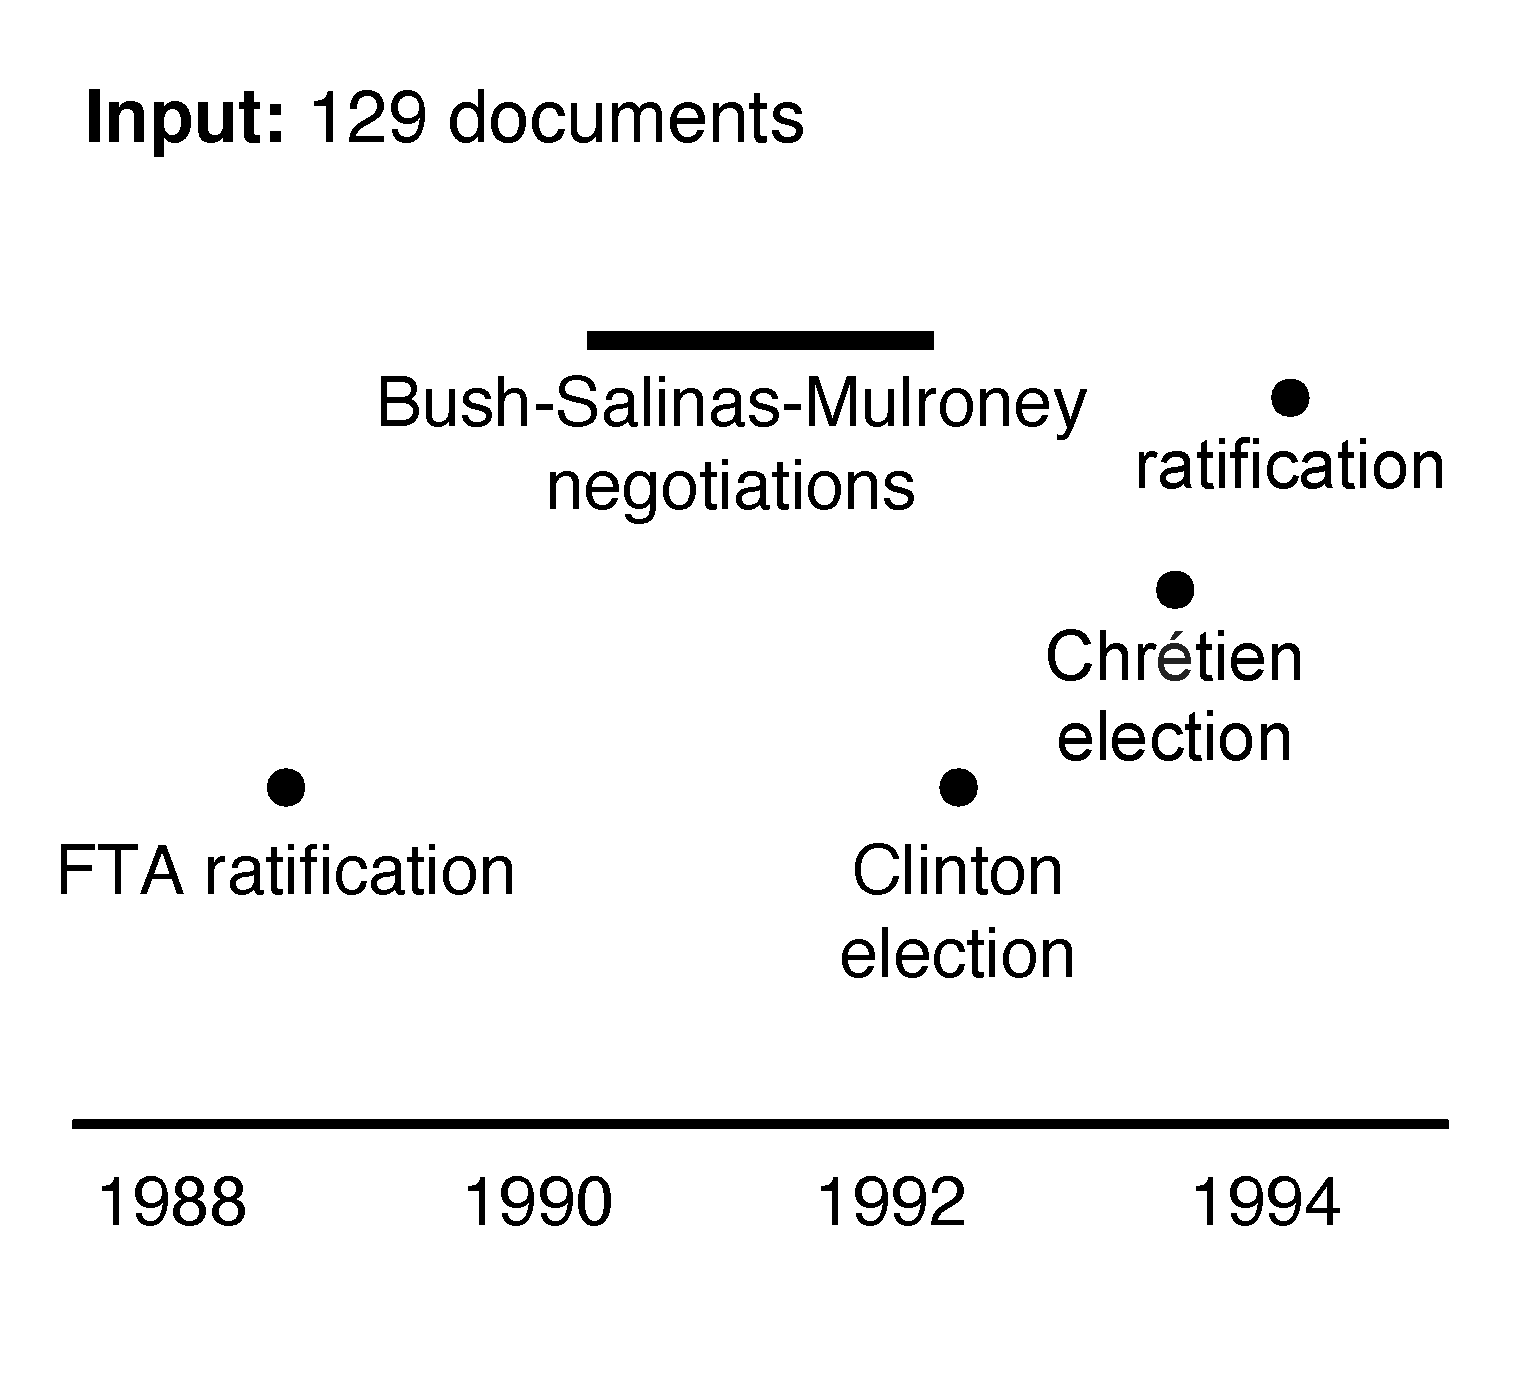
\includegraphics[width=\familypicwidth]{figures/families/timeline.pdf}}
%  \caption{{Visual timeline (Section \ref{s:timeline_family})} \\ 
%  { \centerline{\footnotesize Examples: \cite{LifeLines, TimeLineCurator,james_allan,timelinejs}} }}
%  \label{f:timeline_family}
%\end{subfigure}
\begin{subfigure}{\familypicwidthPlus}
  \centering
  % include second image
  \fbox{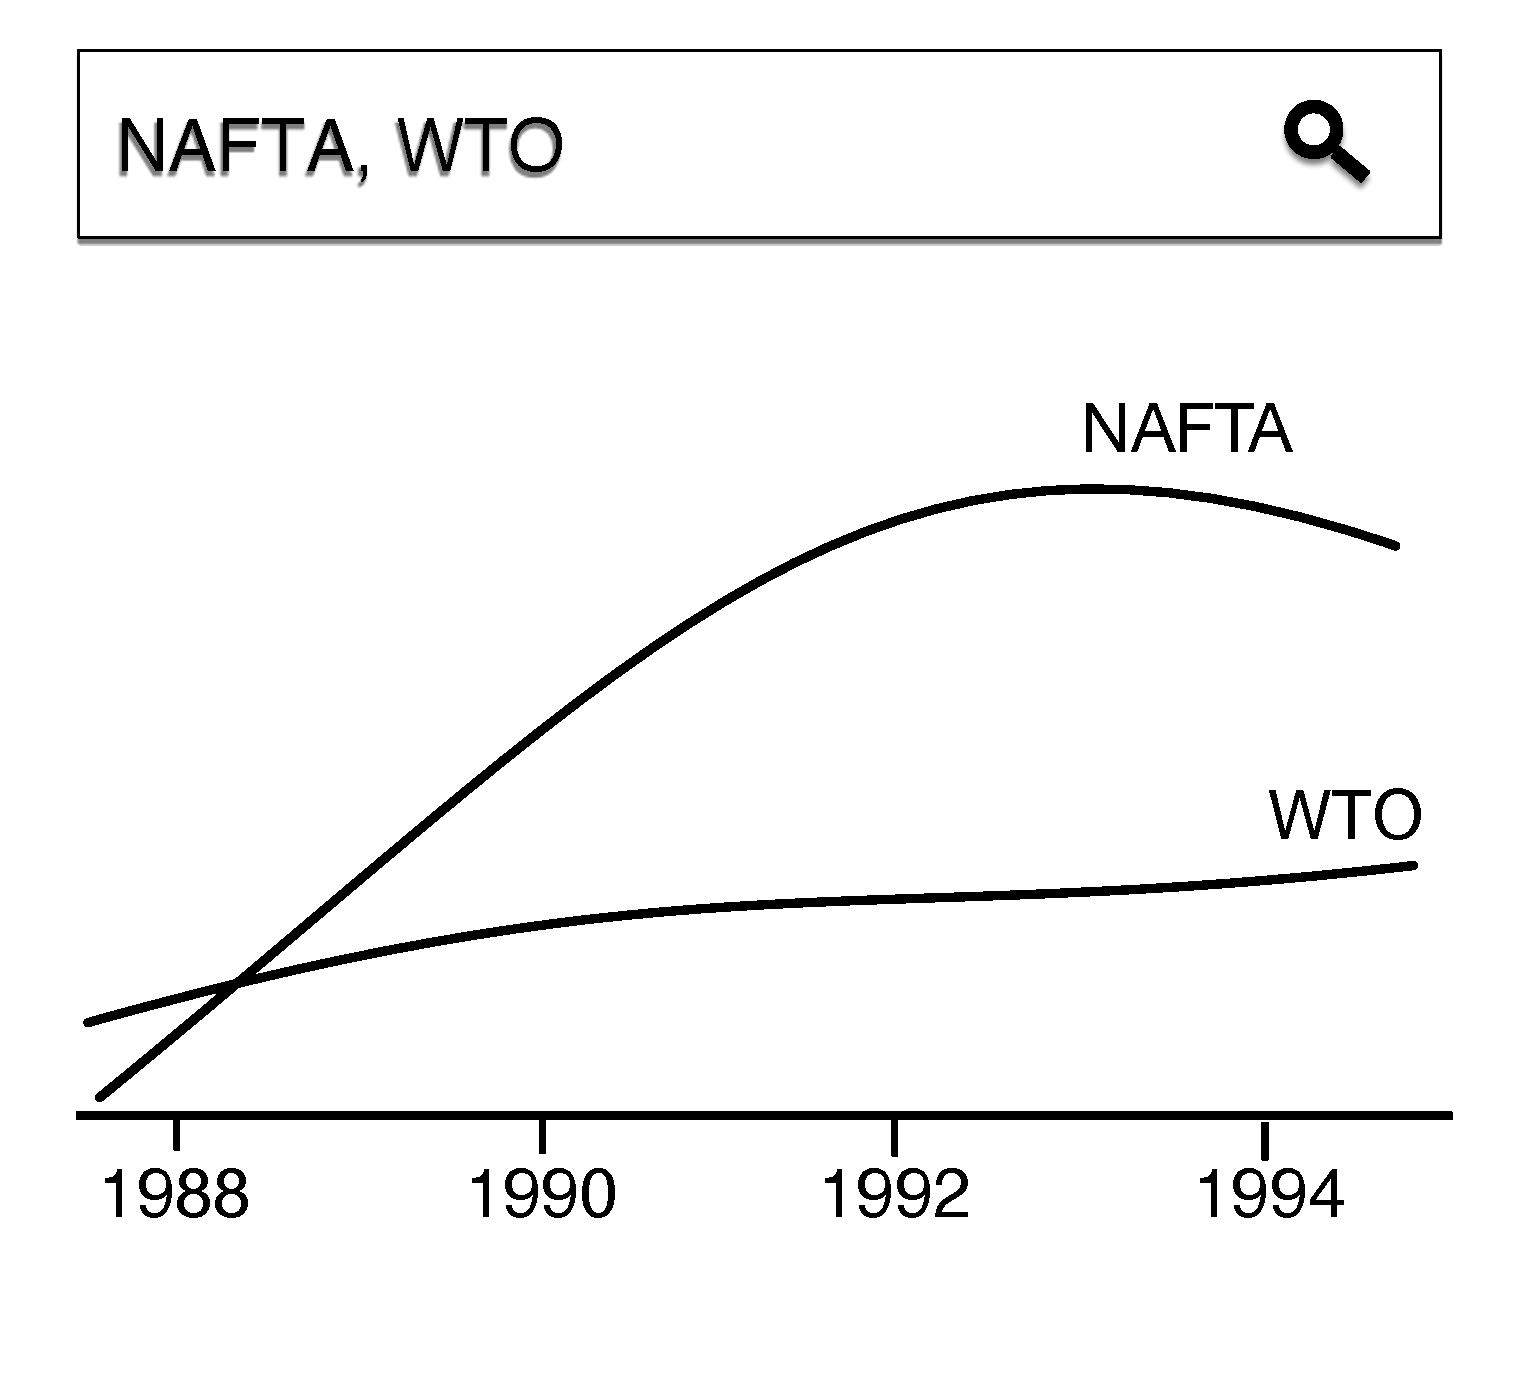
\includegraphics[width=\familypicwidth]{figures/families/timeseries+.pdf}}
  \caption{\hspace{.3cm}{\small Time series plot (Sec.\  \ref{s:time_series_family})} \\ 
  {  \centerline{\footnotesize \hspace{-.4cm} Examples: \cite{ThemeRiver, Michel176, voyant, sotu}}}}
  \label{f:time_series_plus_family}
\end{subfigure} \\ \\    \hline
% % \hspace{-12cm} 
{} \\ 
\begin{subfigure}{\leftwidth}
  {\vspace{\titleoffset}{\textbf{Search} \\  \textbf{patterns}\\ {\small (Sec.\  \ref{s:related_work_search})}}}
\end{subfigure}
\begin{subfigure}{\familypicwidthPlus}
  \centering
  \fbox{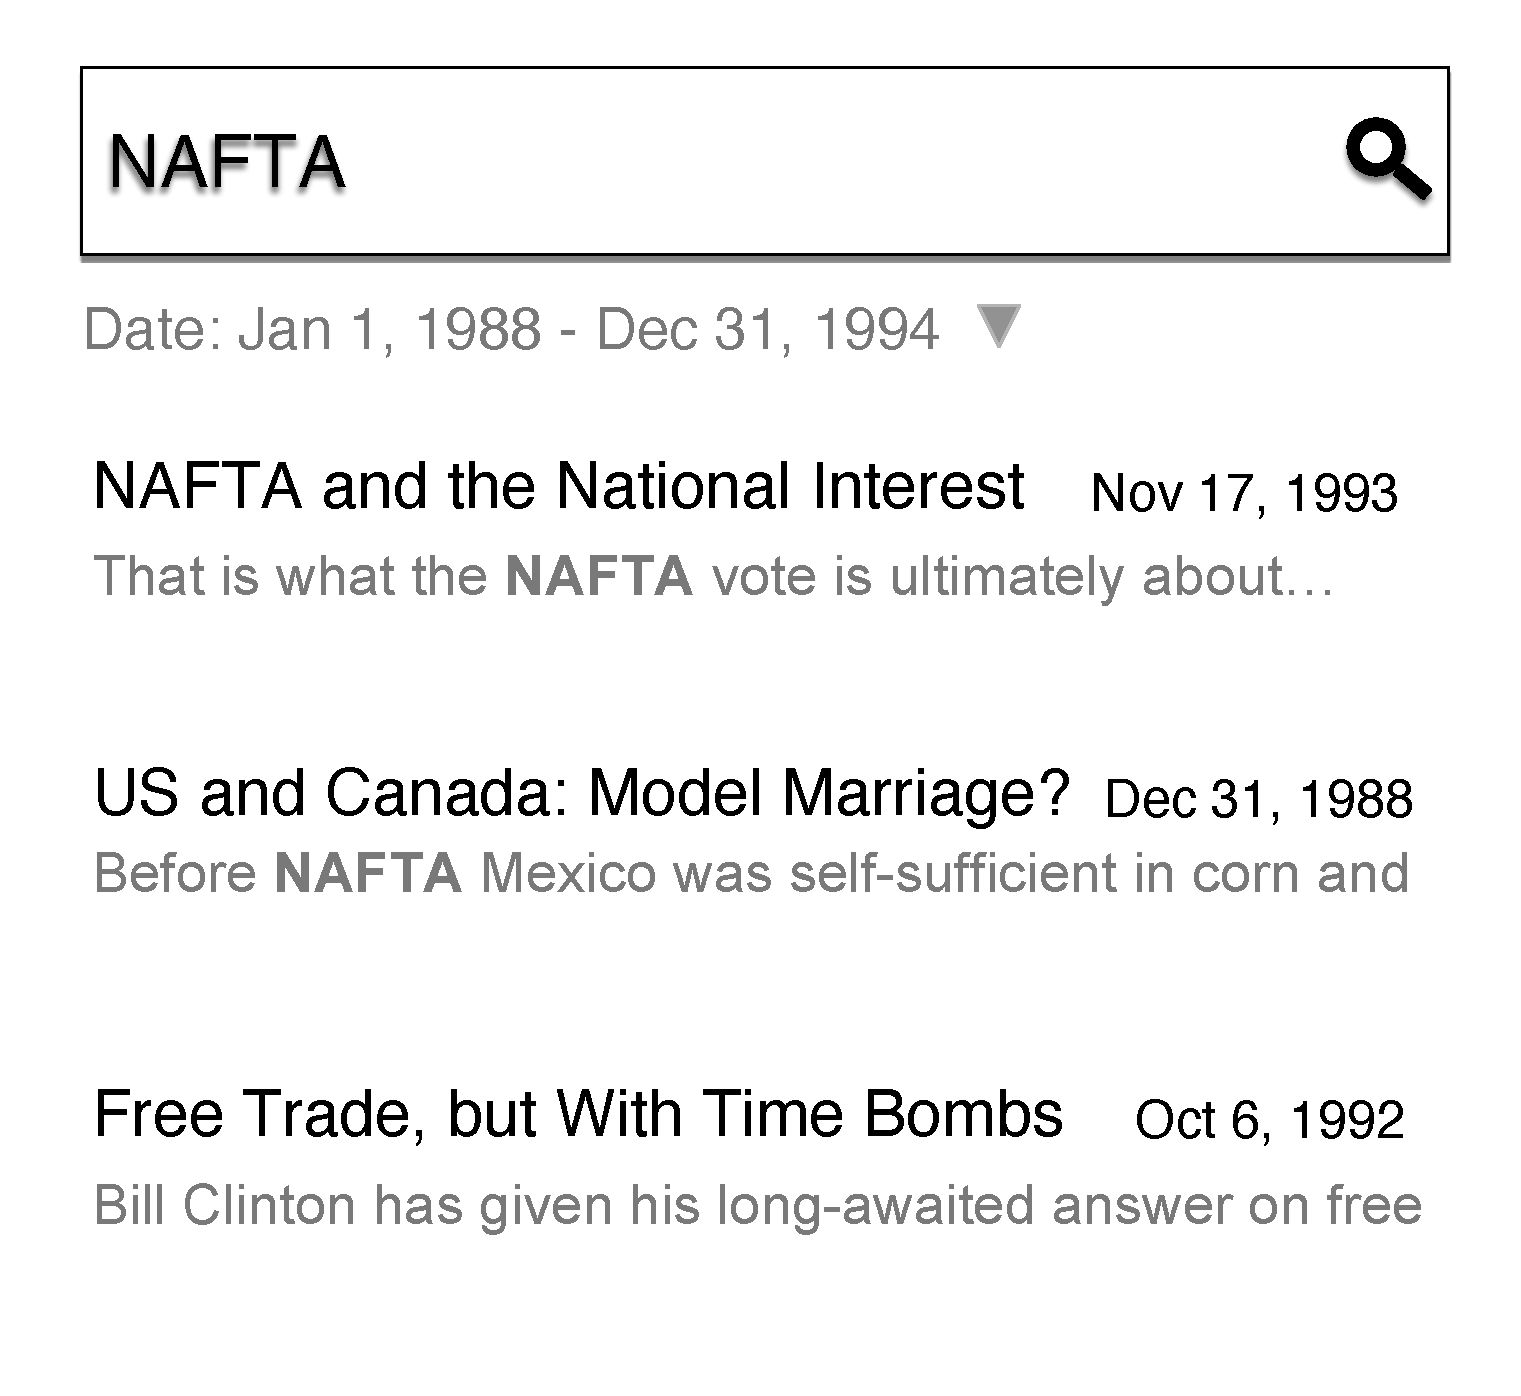
\includegraphics[width=\familypicwidth]{figures/families/search.pdf}}  
  \caption{ {\hspace{.6cm}\small Keyword search (Sec.\  \ref{s:baseline}) } \\ 
   \centerline{\footnotesize Examples: \cite{nytwebsite, TileBars, hotmap, newspapers.com, lucene, voyant}} }
   \label{f:keywordsearch_family}
\end{subfigure}
\begin{subfigure}{\familypicwidthPlus}
  \centering
  \fbox{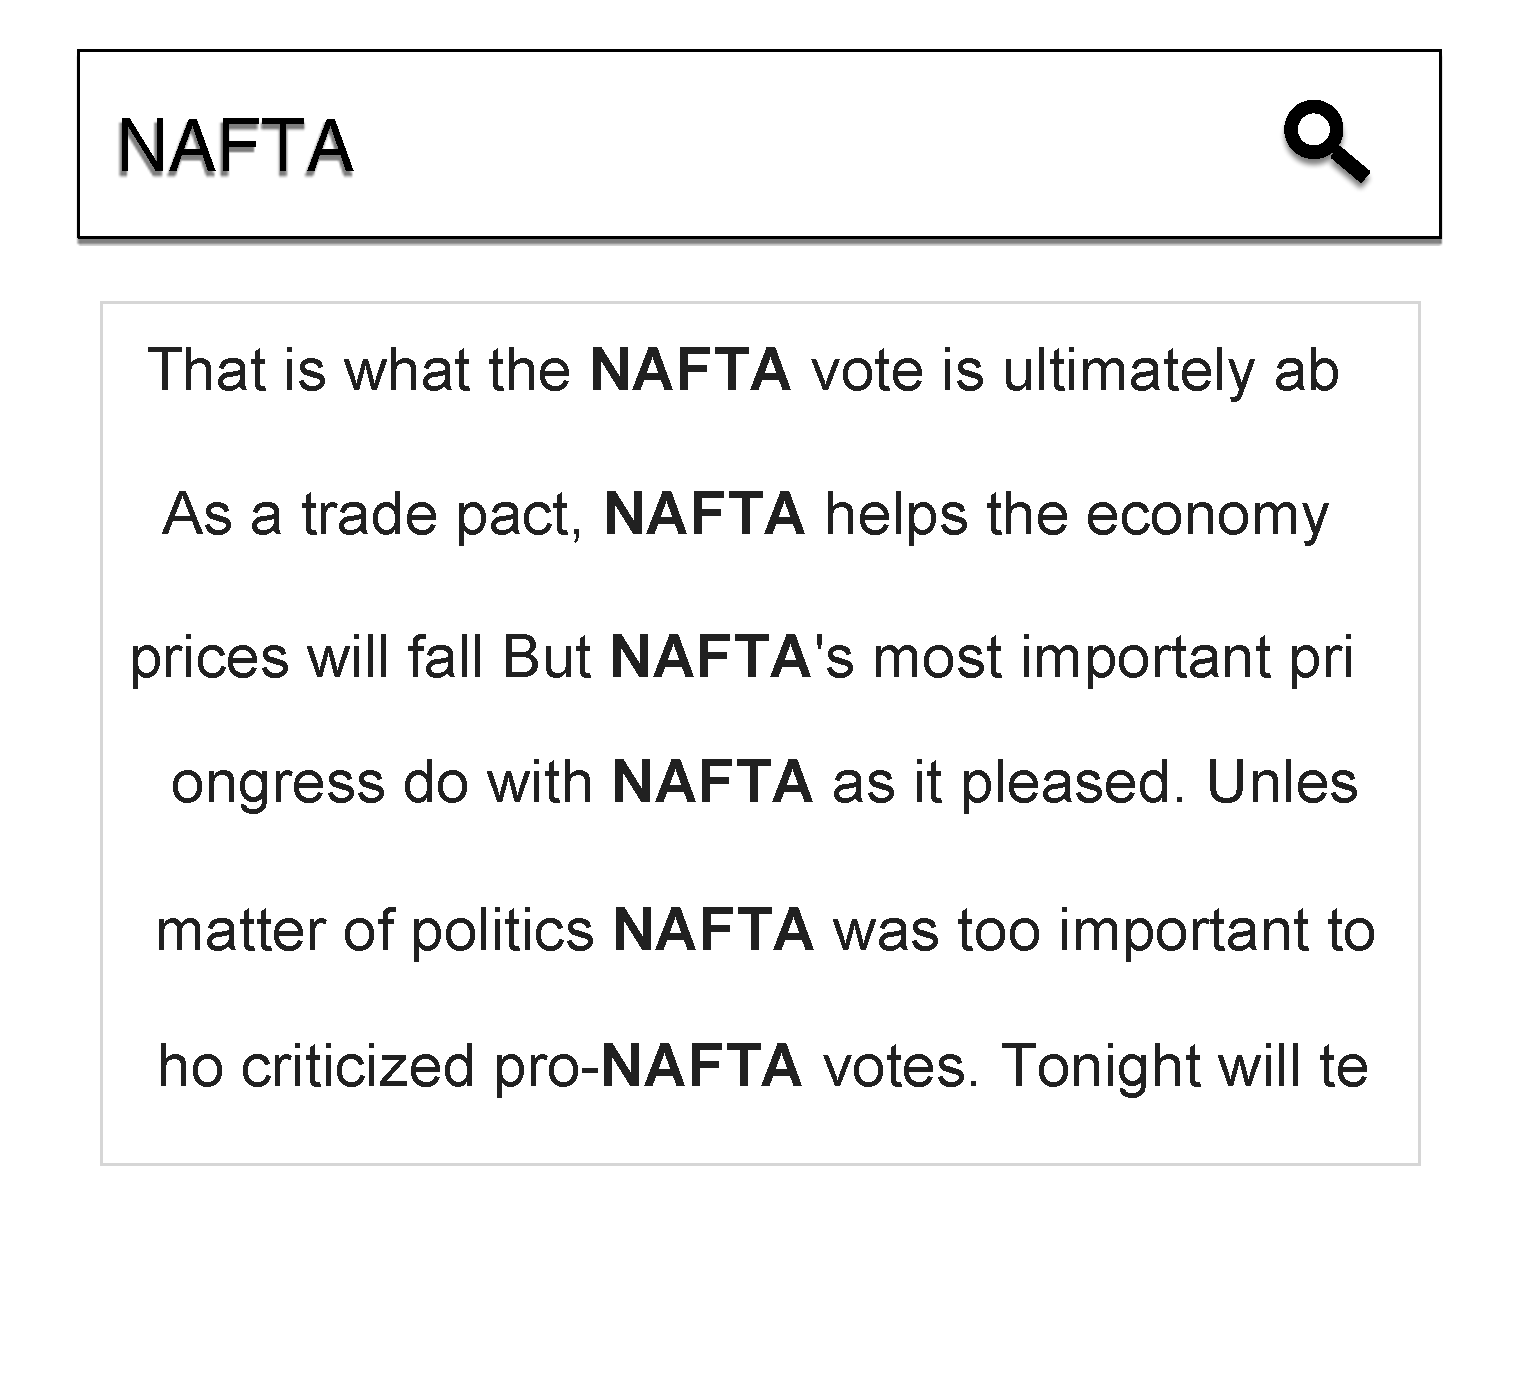
\includegraphics[width=\familypicwidth]{figures/families/kwic2.pdf}}  
  \caption{ {\hspace{.5cm}\small Multi-doc.\ snippet (Sec.\  \ref{s:snippets_family}) } \\ 
  {  \centerline{ \footnotesize Examples:  \cite{Luhn_kwic, oconnor-2014-mitextexplorer, voyant, themail}} }} 
  \label{f:kwic_family}
\end{subfigure} \\ \\ 
\end{tabular}
% push more cites and screenshots to appendix 
% all in one table 
% show what the patterns are clearly and visually consistently 
% adhere to standards in prior work
% 1 X 6 table format (meeting 1/21)
% show all cites 
% ref to sections
% I really like this figure and think it will look terrible w/ heterogenous screenshots
% one page 
% too many cites = line break
% this table holds the most up-to-date version of what systems implement what methods
% \input{samples/tables/family_table}
%\caption{}
\caption[Five major user interface design patterns from prior work]{
\protectWe define five major user interface design patterns from prior work devoted to helping users understand news archives and other corpora (Section \ref{s:related}).
Three of the design patterns focus on helping users gain an overview of archive contents (top two rows).
Two of the design patterns focus on helping the user to search for specific documents or passages from a corpus (bottom row).
Following Tidwell \cite{Tidwell}, this figure presents prototypical wireframes of each design pattern, created by the authors of this work. 
Each example above shows a system presenting results from 129 documents matching the query ``NAFTA'' on a corpus of \textit{New York Times} editorials published between 1988 and 1994. %thesis needs slightly shorter caption for formatting. During thesis compilation families_caption => families_caption_thesis
}\label{f:families_all}
\end{figure}

% http://designinginterfaces.com/firstedition/index.php?page=About_Patterns
% http://www.mit.edu/~jtidwell/common_ground.html => Pointer Shows Affordance
